\begin{frame}{Introducción 01/02}
\justifying
El lienzo le permite dibujar objetos gráficos (por ejemplo, líneas, rectángulos, círculos) y animarlos, el lienzo está integrado en todos los navegadores modernos, por lo que no hay que instalar un software adicional para que los usuarios finales puedan tratar.

{\tiny Web Programming with html5, css, and javascript de John Dean (2019), pág. 570}

Canvas es un elemento HTML incorporado en HTML5 que permite la generación de gráficos dinámicamente por medio del scripting. Entre otras cosas, permite la renderización interpretada dinámica de gráficos 2D y mapas de bits, así como animaciones con estos gráficos. Wikipedia

{\tiny Wikipedia (2020)}
\end{frame}

\begin{frame}{Introducción 02/02}
\justifying
El lienzo le permite dibujar objetos gráficos (por ejemplo, líneas, rectángulos, círculos) y animarlos, el lienzo está integrado en todos los navegadores modernos, por lo que no hay que instalar un software adicional para que los usuarios finales puedan tratar.

{\tiny Web Programming with html5, css, and javascript de John Dean (2019), pág. 570}
\end{frame}

\begin{frame}{Sintáxis básica canvas 01/03}
\justifying
Para usar el lienzo, necesita (1) un elemento del lienzo y (2) llamadas al método JavaScript que dibujan objetos gráficos dentro del área de dibujo del elemento del lienzo. Aquí hay un elemento de lienzo de ejemplo, que crea un área de dibujo rectangular en blanco de 480 píxeles por 250 píxeles en una página web:

\begin{figure}[H]
\centering
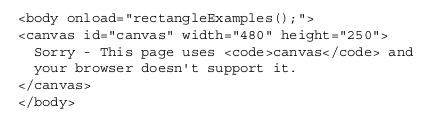
\includegraphics[scale=0.5]{Section_Files/images/Sec01/01.png}
\end{figure}


{\tiny Web Programming with html5, css, and javascript de John Dean (2019), pág. 571}
\end{frame}

\begin{frame}{Sintáxis básica canvas 02/03}
\justifying
Después de que se carga la página web, el evento onload se activa y llama a la función rectangleExamples, que dibuja formas rectangulares dentro del área de dibujo del lienzo. Examinaremos la función rectangleExamples en la siguiente sección. Como habrás adivinado, el atributo id del elemento del lienzo permite que la función acceda al objeto del lienzo. Tenga en cuenta el texto que aparece entre las etiquetas del elemento del lienzo. Ese es el contenido alternativo. Se muestra cuando el navegador del usuario no admite el elemento de lienzo. Si necesita admitir navegadores antiguos, debe incluir dicho contenido alternativo, pero dado que todos los navegadores modernos admiten lienzo,

{\tiny Web Programming with html5, css, and javascript de John Dean (2019), pág. 571}
\end{frame}

\begin{frame}{Sintáxis básica canvas 03/03}
\justifying
Hay dos tipos de comandos de dibujo de lienzo: los que dibujan imágenes bidimensionales y los que dibujan imágenes tridimensionales. Vamos a mantener las cosas simples y seguir con las imágenes bidimensionales. Para crear imágenes bidimensionales, recupera el contexto bidimensional del lienzo de esta manera:

\begin{figure}[H]
\centering
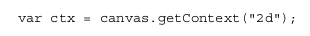
\includegraphics[scale=0.5]{Section_Files/images/Sec01/02.png}
\end{figure}

Normalmente, debe mantenerse alejado de las abreviaturas oscuras para nombres de variables, pero ctx es una abreviatura estándar para el contexto de un lienzo.

{\tiny Web Programming with html5, css, and javascript de John Dean (2019), pág. 572}
\end{frame}

